\subsection{Setup}

\begin{figure}[h]
\centering
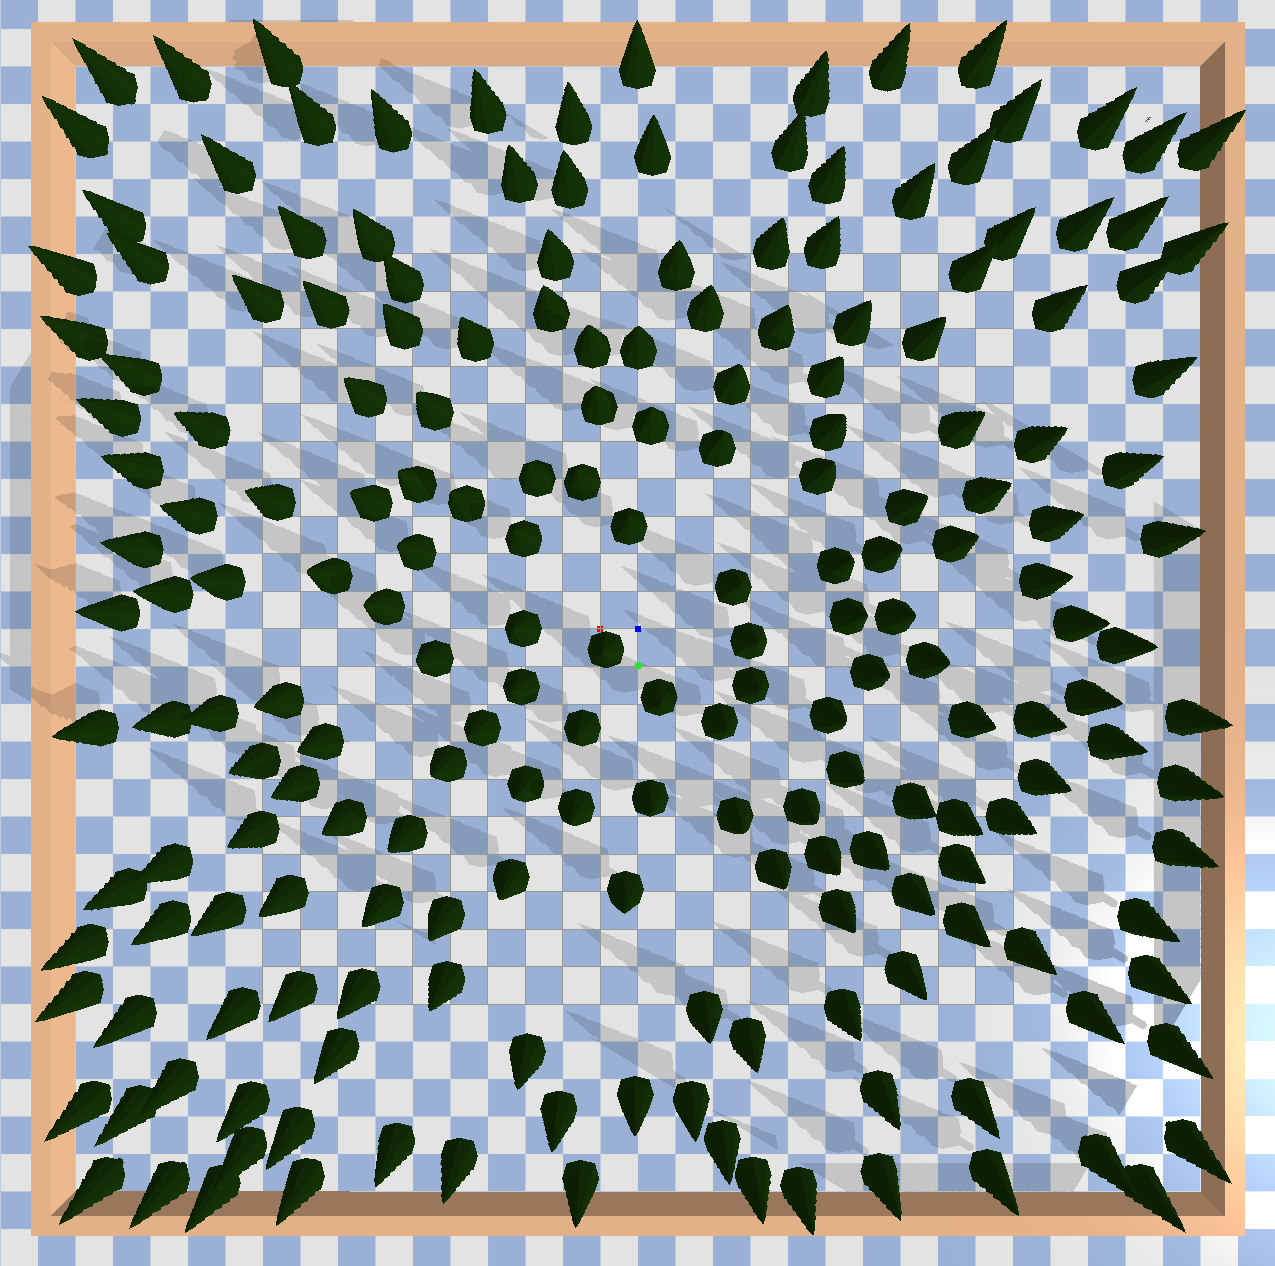
\includegraphics[width=0.5\textwidth]{images/SimulationImage.png}
\caption{Simulation (top view)}
\end{figure}


The simulation uses pybullet for physics and few control methods adapted from gym-pybullet-drones. Important parameters used for experimenting are - number of drones, number of trees and area size. For the most part we've used $3$ drones for exploring a forest area of $900m^2$ with $200$ trees (obstacles) as shown in Fig. 1. \\

\begin{figure}[h]
\centering
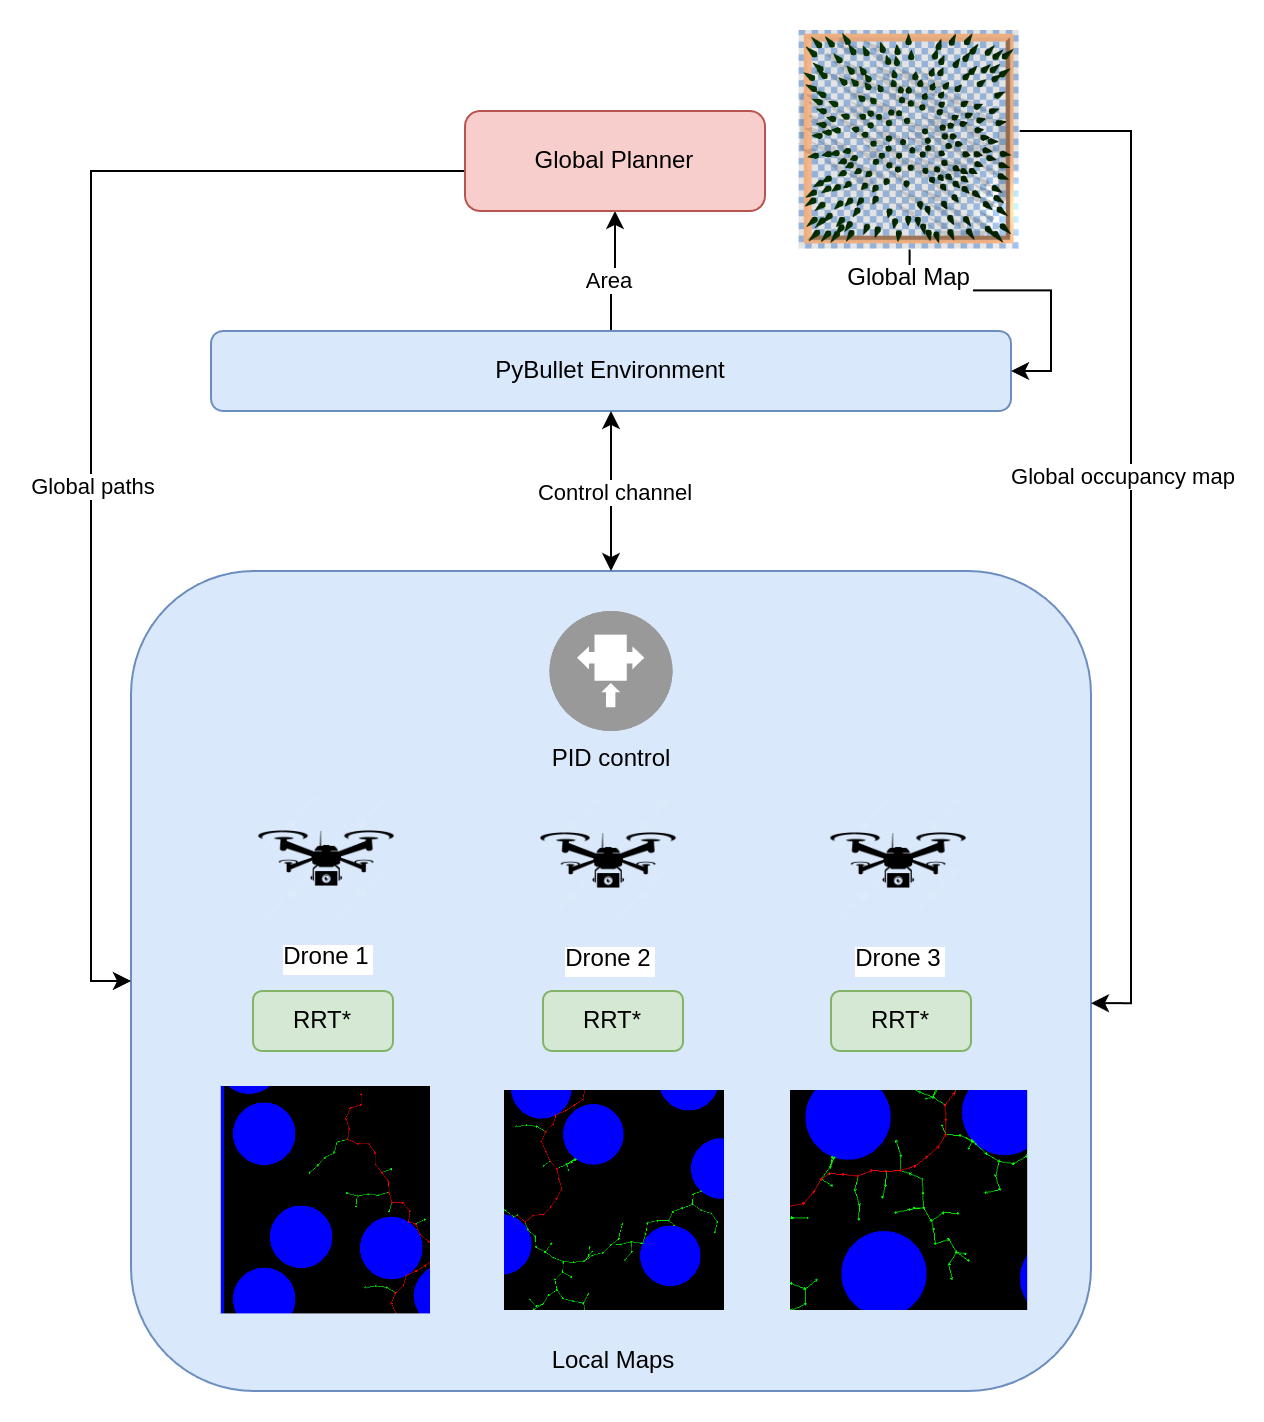
\includegraphics[width=0.5\textwidth]{images/arch_diag.png}
\caption{Architecture diagram}
\end{figure}

Other parameters include simulation frequency set at 48Hz. In each step/loop the next action is either executed or sampled (planned) for a drone.

Fig 2. represents a high level overview of how all processes tie in together to compute and execute a obstacle free path.

\subsection{Results}
\begin{figure}[h]
\centering
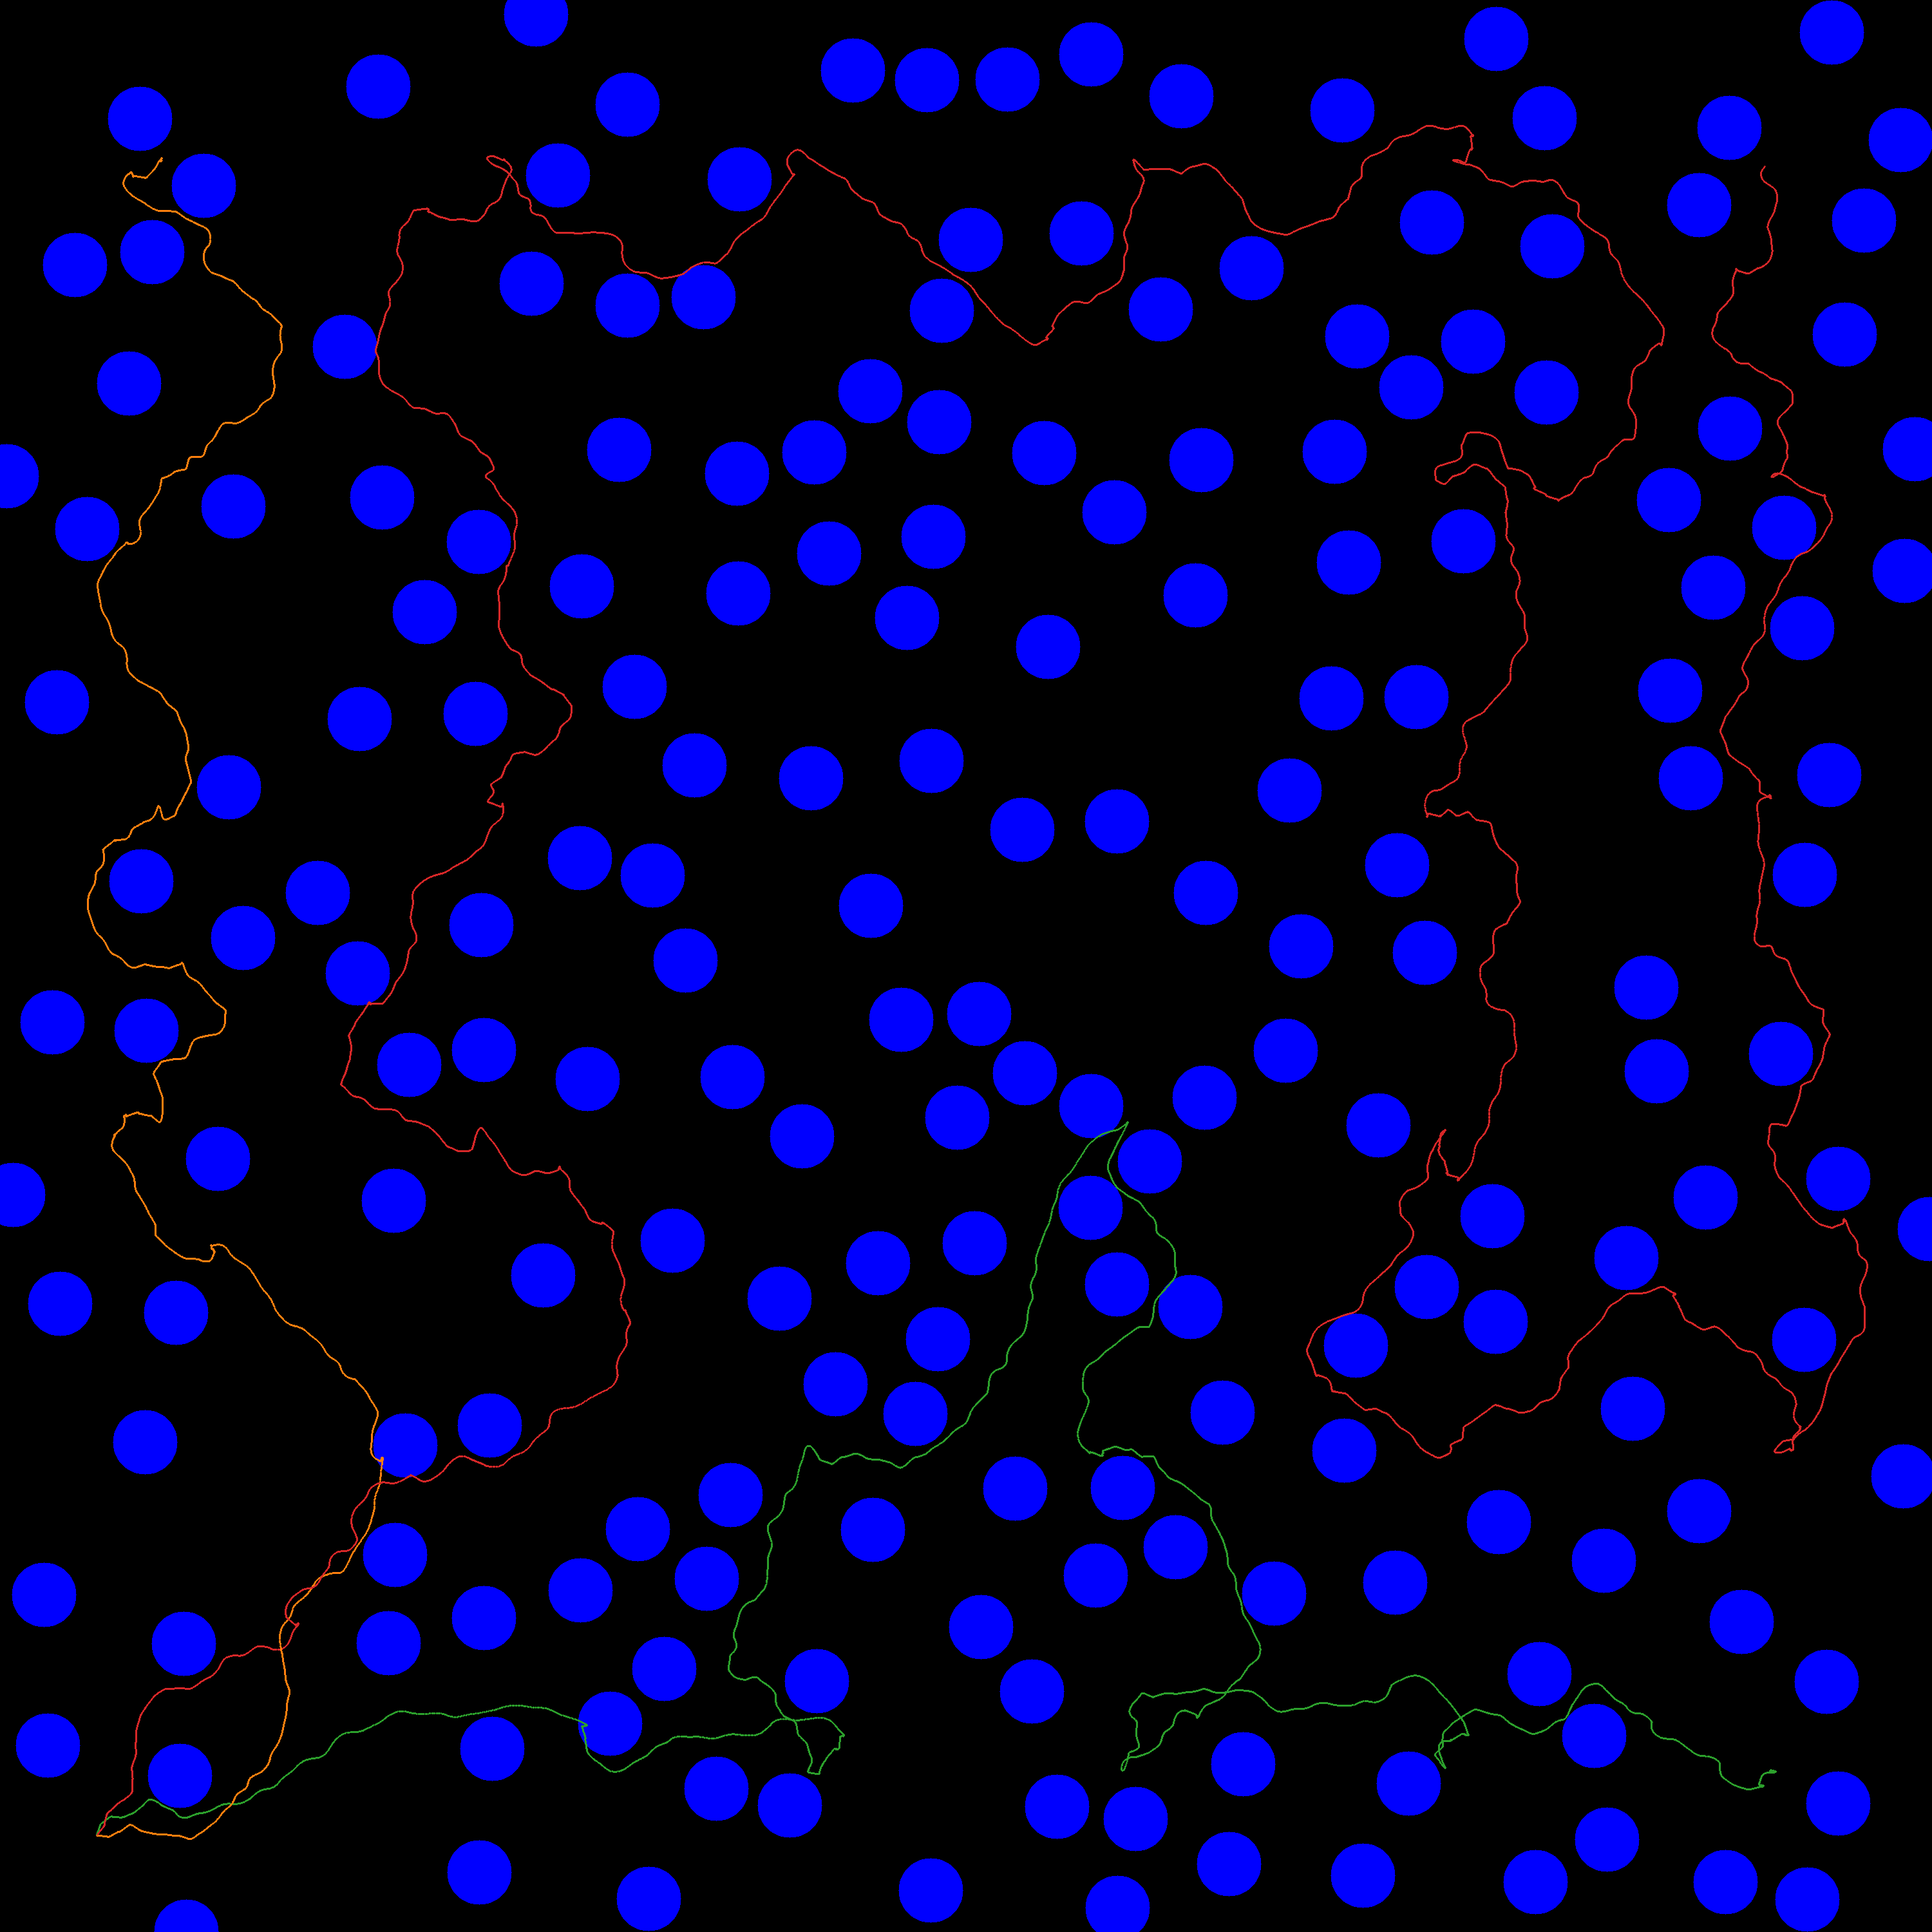
\includegraphics[width=0.5\textwidth]{images/preview_map_frame_11193.png}
\caption{Occupancy map on a 30 x 30 m area}
\end{figure}

\begin{figure}[h]
\centering
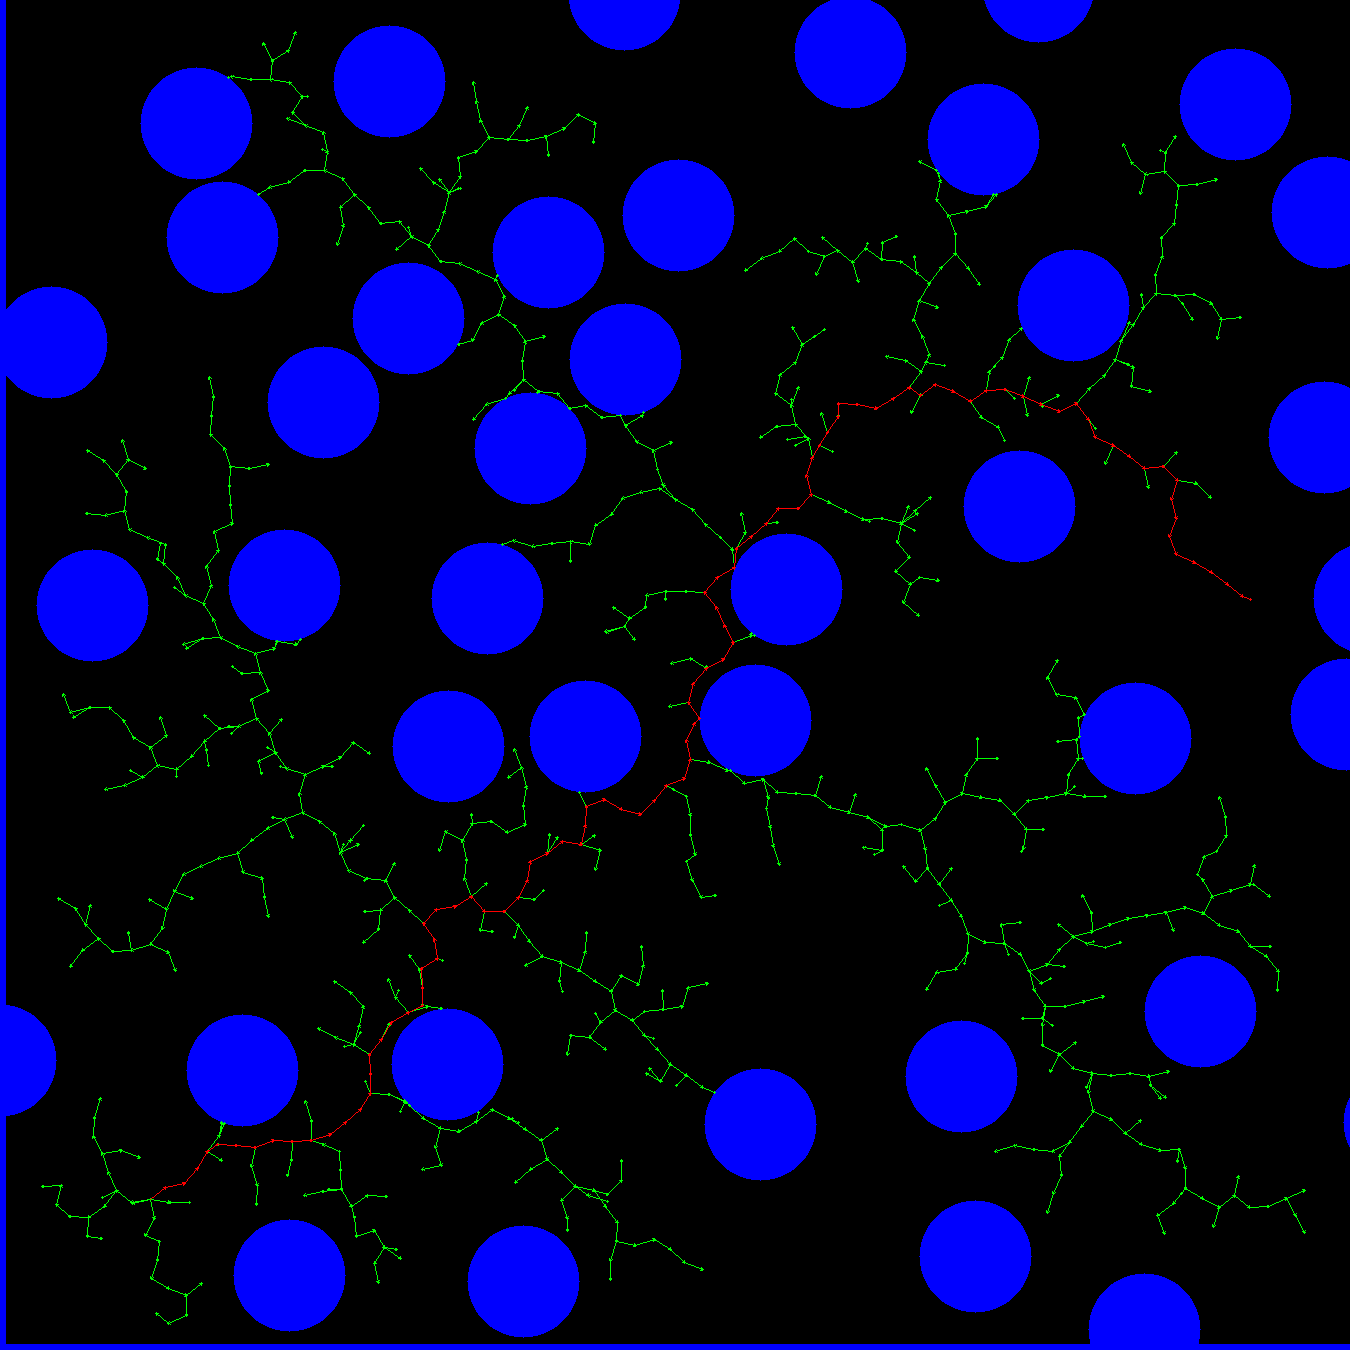
\includegraphics[width=0.5\textwidth]{images/rrt_drone_2_iter_0.png}
\caption{RRT on a local occupancy map}
\end{figure}

This \href{https://www.youtube.com/watch?v=JBWNEh0Fis4&ab_channel=ShantnavAgarwal}{video} shows drones navigating in the aforementioned setup.\\

Fig. 3 shows paths followed by each drone to explore the map using paths provided by global path planner and RRT algorithm, which took 8 hours in simulation time (3 mins in practice). \\

%[picture] shows the simulation running in a smaller area of $400m^2$ with $100$ trees took x mins. \\

Fig. 4 shows the RRT trees in a local map. As shown the drone doesn't have to know its final goal postion and such a series of local maps can guide the drone towards the goal while offering benefits of faster computation.